\documentclass[12pt]{article}

\usepackage{amssymb,amsmath}
\usepackage[margin=1.0in]{geometry}
\usepackage{fancyhdr} % required for custom header
\usepackage{graphicx}
\usepackage{listings}
\usepackage{courier}
\usepackage[usenames,dvipsnames]{color}

%set up the header
\pagestyle{fancy}
\lhead{Trever Hines}
\chead{El Mayor Postseismic}
\rhead{\today}

\setlength{\headheight}{15pt}
\renewcommand\headrulewidth{1.0pt} % Size of the header rule

%% Title
%%------------------------------------------------------------------------------
\title{	
El Mayor Postseismic
\author{Trever Hines}
\rule{\headwidth}{1.0pt}
}


\begin{document}
\maketitle
\section*{Introduction}
\begin{figure}
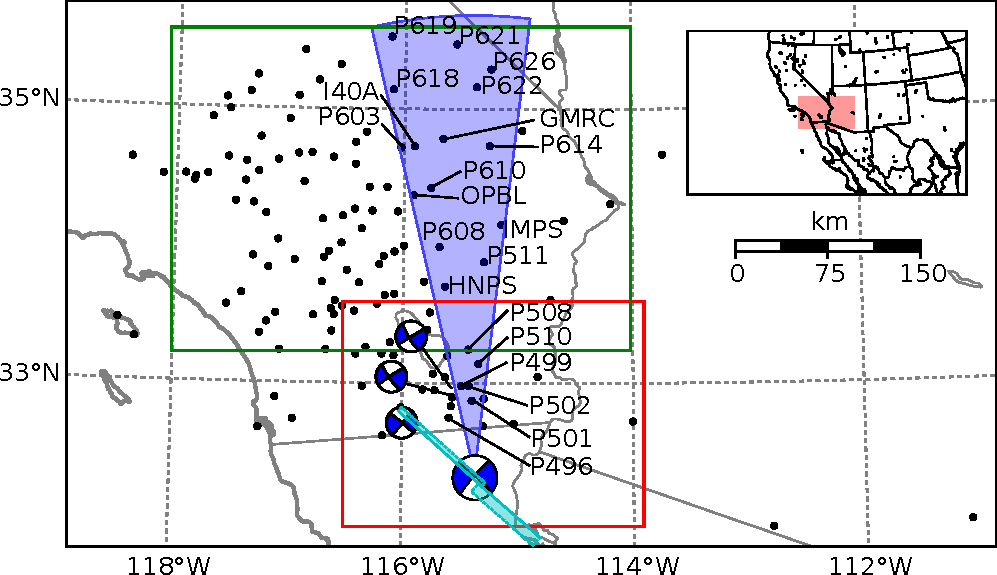
\includegraphics[scale=0.2]{Figures/ContextMap}
\centering
\caption{test}
\end{figure}
  sdfdf
    
Previous studies which have modeled postseismic deformation following the El Mayor-Cucapah earthquake include \cite{Pollitz2012}, \cite{Gonzalez-ortega2014}, \cite{Spinler2015}, and \cite{Rollins2015}. \cite{Gonzalez-ortega2014} was able to describe five months of near field ($\lesssim 50$ km from the epicenter) postseismic defomation observed by InSAR and campaign GPS with afterslip and fault contraction on the coseismically ruptured fault. \cite{Gonzalez-ortega2014} also noted that their preferred model underestimated the GPS displacements for stations $\gtrsim 25$ km from the rupture and suggested that it could be the result of unmodeled viscoelastic relaxation.  Using continuous GPS stations within 200 km of the El Mayor-Cucapah epicent, which consists mostly of stations north of the US-Mexico border, \cite{Rollins2015} found that three years of postseismic deformation can be adequately explained by afterslip in an elastic lithosphere, albeit with an implausibly large amount of afterslip inferred on the least constrained southern most fault segment which may be acting as a proxy for distributed relaxation in the lower crust or upper mantle. In this paper, we reiterate this finding by \cite{Rollins2015} and note that a purely elastic dislocation model is incapable of describing deformation observed at GPS stations greater than ~200 km from the El Mayor-Cucapah epicenter.  

Given the inability to describe both near and far field deformation with fault slip in an elastic lithosphere, \cite{Pollitz2012}, \cite{Rollins2015} and \cite{Spinler2015} have explored viscoelastic relaxation in the lower crust and upper mantle as a potential deformation mechanism. The lithospheric rheology is largely unknown and so modeling postseismic deformation with viscoelastic relaxation requires one to assume a rheologic model and find the best fitting model parameters, which is generally a computationally expensive nonlinear inverse problem. Consequently, a simplified structure for the lithosphere must be made to minimize the number of rheologic parameters that need to be estimated.  For example, it is commonly assumed that the lithosphere consits of only three homogeneously Maxwell viscoelastic layers, which may be an inadequate representation of the lithosphere \cite{Hines2013}\cite{Riva2009}. Additionally, it is necessary to make simplifying assumptions about the nature of afterslip.  For example \cite{Pollitz2012} and \cite{Spinler2015} assumed that afterslip does not persist beyond six months and one year respectively and subsequent displacements were assumed to be the result of only viscoelastic relaxation. However, numerous observations of interseismic fault creep has been recognized in this and similar tectonic settings and it has been speculated that such creep can be initiated as a postseismic process \cite{Cakir2012} \cite{Cetin2014}.
We are unaware of any oIn this study, we therefore do not make to implicit assumption that afterslip terminates after a given amount of time.  Indeed, the preferred viscoelastic model from \cite{Pollitz2012} underpredicts near field velocities, which could be indicative of unmodeled continued afterslip.

All of the aforementioned studies model displacements observered at stations within 200 km of the El Mayor-Cucapah epicenter, while postseismic deformation in this region following previous earthquakes of similar magnitude has been observed at distances extended out to about 300 km \cite{Freed2007a}. In the present study we examine stations within 400 km of the El Mayor-Cucapah epicenter, which turns out to be crucial for discerning the postseismic deformation mechanism.

Clearly, both afterslip and viscoelastic relaxation are involved in postseismic deformation neglecting to model one of these deformation mechanisms could result in a biased estimate of the other.  In this paper we use the inverse method described in \cite{Hines2015} to estimate the afterslip an effective viscosity necessary to describe the transience postseismic deformation over the first ten months after the El Mayor-Cucapah earthquake. We then form a suite of models which have various lithospheric rheologies but viscosities that are consistent with the effective viscosity estimated from the early postseismic deformation. Of the suite of models tested, we find that five years of postseismic deformation can be explained by a combination of sustained afterslip on the coseismicly ruptured fault and a Zener rheology upper mantle with viscosity that decays from $4\times10^{18}$ to $1\times10^{18}$ Pa s. 


\section*{Data Processing}

We use continuous GPS position time series provided by University Navstar Consortium (UNAVCO) for Plate Boundary Observatory (PBO) stations within a 400 km radius about the El Mayor-Cucapah epicenter. Our analysis is on the coseismic and postseismic deformation resulting from the EMC earthquake, which we collectively describe as $u(t)$. We consider GPS position time series, $u_\mathrm{obs}(t)$, to be the superposition of $u(t)$, secular tectonic deformation, annual and semi-annual fluctuations, and coseismic offsets from sigificant earthquakes over the time span of this study.  The June 14, 2010 Mw5.8 Ocotillo earthquake and the August 26, 2012 Brawley swarm, which consisted of a Mw5.5 and Mw5.3 event, are the only earthquakes after the EMC earthquake that produced noticeable offsets recorded by GPS. Although the Ocotillo earthquake had its own series of aftershocks (Haukson), neither earthquake produced transient deformation that is detectable with GPS. We thus model $u_\mathrm{obs}(t)$ as 

\begin{equation}\label{TimeSeriesModel}
  \begin{split}  
    u_\mathrm{obs}(t) = &u(t) + c_0 + c_1t + \\
                       &c_2\sin(2\pi t) + c_3\cos(2\pi t) + c_4\sin(4\pi t) + c_5\cos(4\pi t) + \\
                       &c_6H(t-t_\mathrm{oc}) + c_7H(t-t_\mathrm{bs}) + \epsilon.
  \end{split}
\end{equation}
Where $t_\mathrm{oc}$ and $t_\mathrm{bs}$ are the times of the Ocotillo earthquake and Brawley swarm respectively, $H(t)$ is the Heaviside function, $c_0$ through $c_7$ are unknown coefficients, and $\epsilon$ is noise with zero mean and variance that is assumed known.

Stations which recorded signals that clearly cannot be described by the aforementioned processes are not included in our analysis. This includes stations in the Los Angeles basin, which record deformation that is largely anthropogenic. In order to ensure an accurate estimation of the secular deformation, we only use stations that were installed at least six months prior to El Mayor-Cucapah earthquake. While several stations were installed after the EMC earthquake to improve the spatial resolution of postseismic deformation \cite{Spinler2015}, our inverse method uses postseismic displacements rather than velocities (e.g. ...), which requires the knowledge of the stations preseismic position. Despite our inability to utilize potentially rich data, we prefer to use postseismic displacements rather than potentially dubious estimates of postseismic velocities.

The October 16, 1999 Hector Mine earthquake, which occurred within our study region about 270 km north of the EMC epicenter, has produce transient postseismic deformation which we do not wish to model either mechanically or through empirical line fitting. We thus restrict our analysis to deformation observed six years after the Hector Mine earthquake, past which point postseismic deformation for nearfield sites occurs at an approximately steady rate \cite{Savage2009}. When considering stations further away from the Hector Mine epicenter, postseismic transience persists for only about two years \cite{Spinler2015}.

We do not assume a parametric form for $u(t)$, (e.g. \cite{Rollins2015}), but rather we model $u(t)$ as integrated Brownian motion, so that 
\begin{equation}
    \dot{u}(t) = \sigma^2\int_0^t w(s) ds.
\end{equation}    

where $w(t)$ is white noise and the variance of $\dot{u}(t)$ increases linearly with time by a factor of $\sigma^2$. We use a
Kalman filtering approach to estimate $u(t)$ and the unknown parameters in eq. \ref{TimeSeriesModel} which we describe now.  In the context of Kalman filtering, our time varying state vector is
\begin{equation}
    \mathbf{X}(t) = [u(t),\dot u(t), c_0, ..., c_7]
\end{equation}
and eq. \ref{TimeSeriesModel} is the observation function which maps the state vector to the GPS observations. We initiate the Kalman filter by assuming a prior estimate of $\mathbf{X}(t)$ at time $t_0$ which has a sufficiently large covariance to effectively make our prior uninformed.  For each time epoch, $t_i$, Bayesian linear regression is used to incorperate GPS derived estimates of displacement with our prior estimate of the state, $\mathbf{X}_{i|i-1}$, to form a postserior estimate of the state, $\mathbf{X}_{i|i}$, which has covariance $\mathbf{\Sigma}_{i|i}$.  

We then use the posterior estimate of the state at time $t_i$ to form a prior estimate of the state at time $t_{i+1}$ through the transition function
\begin{equation}\label{predict}
  \mathbf{X}_{i+1|i} = \mathbf{F}_{i+1}\mathbf{X}_{i|i} + \mathbf{\delta}_{i+1} 
\end{equation}
where 
\begin{equation}
  \mathbf{F}_{i+1} = 
  \left[
  \begin{array}{ccc}
    1           & (t_{i+1} - t_i) & \mathbf{0}\\
    0           & 1              & \mathbf{0}\\
    \mathbf{0}  & \mathbf{0}     & \mathbf{I}
  \end{array}
  \right]
\end{equation}
and $\mathbf{\delta}_{i+1}$ is the process noise, which has zero mean and covariance described by
\begin{equation}
  \mathbf{Q}_{i+1} = 
  \sigma^2 \left[
  \begin{array}{ccc}
  \frac{(t_{i+1} - t_i)^3}{3} & \frac{(t_{i+1} - t_{i})^2}{2} & \mathbf{0}\\
  \frac{(t_{i+1} - t_i)^2}{2} & (t_{i+1} - t_{i}) & \mathbf{0}\\ 
  \mathbf{0} & \mathbf{0} & \mathbf{0}
  \end{array}
  \right].
\end{equation}

The covariance of the new prior state, $\mathbf{X}_{i+1|i}$, is then described by
\begin{equation}
  \mathbf{\Sigma}_{i+1|i} = \mathbf{F}_{i+1}\mathbf{\Sigma}_{i|i}\mathbf{F}^T_{i+1} + \mathbf{Q}_{i+1}.
\end{equation}

This process is repeated for each of the $N$ time epochs at which point we use Rauch-Tung-Striebel smoothing to find $X_{i|N}$, which is an estimate of the state at time $t_i$ that incorporates all $N$ GPS observation.  Our final estimates of $u(t)$ are used in subsequent analysis, while the remaining components of of the state vector are considered nuisance parameters. In the interests of computational tractability, we down sample our smoothed time series from daily solutions down to weekly solutions.

The smoothness of $u(t)$ is controlled by the chosen value of $\sigma^2$, which describes how rapidly we expect the postseismic signal to vary over time. As one endmember, setting $\sigma^2$ equal to zero will effectively result in modeling $u(t)$ as a straight line. The other endmember, where $\sigma^2$ is infinitely large, will result in $u(t)$ fitting what is obviously noise in the data. While one can use a maximum likelihood based approach to picking $\sigma^2$ (e.g. \cite{Segall1997}), we rather take a subjective approach and choose a value for $\sigma^2$, which is used when filtering time series for each station, that is just large enough to faithfully describes the early rapid rate of postseismic deformation at the most near field station in our study, P496.  This ensures that $\sigma^2$ will be sufficiently large so that our estimate of $u(t)$ does not smooth out potentially valuable postseismic signla.  Figure 1 shows the .... While formal errors are estimated for $u(t)$ it is important to know that the true uncertainty in $u(t)$ is much larger due to assumptions made in formulating eq. (1).  For example, we assume that the background rate of tectonic deformation can be approximated a linear rate, while is appears to hold true based on inspection of the time series, mechanical models would suggest this to not be true on earthquake cycle timescales 

             

We illustrate the effect of filtering in figure ().  We assume a constant $\sigma^2$ for each station, which is chosen to be just large enough for the earliest transient deformation at the most nearfield site, P496?, to be faithfully described by the filtered solution.

Cite Freed 2007 for far reaching postseismic after Landers/Hector Mine.

\section*{Observations}

\section*{Prior Studies}

\section*{Postseismic Modeling}

We use a fault geometry from \cite{Wei2011}, which was determined using teleseismic, GPS, and InSAR data.  

After the El Mayor-Cucapah earthquake, additional GPS stations were installed In Baja California to record postseismic deformation with better spatial coverage.  Two of the stations PTAX and PHJX were installed near the epicenter in the Cucapah Mountains.  We do not include these two stations in our analysis because the geometry of the faults that ruptured during the earthquake is more complicated than our assumed fault geometry \cite{Oskin2012} \cite{Fletcher2014} and the near field stations would be most sensitive to error in our geometry. We also leave of these near field stations in order to avoid any near field processes which we do not consider in this paper \cite{Gonzalez-ortega2014}. Numerous stations exhibit extraneous signals which can be 

\section*{Rheological constraints}

\section*{Results}
\section*{Acknowledgements}

This material is based on EarthScope Plate Boundary Observatory data services provided by UNAVCO through the GAGE Facility with support from the National Science Foundation (NSF) and National Aeronautics and Space Administration (NASA) under NSF Cooperative Agreement No. EAR-1261833.

\bibliographystyle{apalike}
\bibliography{mybib}

\end{document}

